
\documentclass{article}
\usepackage{graphicx} % Required for inserting images

\usepackage{geometry}
\usepackage{array}
\usepackage{amsmath}
\usepackage{amsfonts}
\usepackage{amssymb}

\geometry{margin=1in}

\title{Evolutionary Multiobjective Optimization Software: NSGAII}
\author{Daniel Amadori}

\begin{document}

\maketitle

\section*{Abstract}
This report investigates the application of the nondominated sorting genetic algorithm (NSGA-II) to solve the ZD4 problem using multiobjective evolutionary optimization. The study explores various combinations of parameters, specifically population size and mutation rate, to analyze their impact on algorithm convergence. The evaluation is based on the hypervolume metric, providing insights into the balance between exploration and exploitation in the optimization process.

\section{Introduction}
Multiobjective evolutionary algorithms (MOEAs) play a crucial role in solving complex optimization problems with multiple conflicting objectives. This report focuses on the NSGA-II, a nondominated sorting-based MOEA that addresses computational complexity, nonelitism, and sharing parameter issues commonly associated with such algorithms.

\subsection{Problem Definition}
The NSGA-II algorithm will be employed to tackle the ZD4 problem, and for each combination of parameters tested, figures depicting the non-dominated final front and convergence curves of the hypervolume indicator will be presented.
\begin{table}[h]
    \centering
    \renewcommand{\arraystretch}{1.5} % Adjust the spacing between rows
    \begin{tabular}{|c|c|c|c|}
        \hline
        $n$ & Variable Bounds & Objective Functions & Optimal Solutions \\
        \hline
        10 & $x_1 \in [0, 1]$, & $f_1(x) = x_1$, & $x_1 \in [0, 1]$, \\
           & $\forall i \in \{2, \ldots, n\}: x_i \in [-5, 5]$ & $f_2(x) = g(x) \left(1 - \sqrt{\frac{x_1}{g(x)}}\right)$, & $\forall i \in \{2, \ldots, n\}: x_i = 0$ \\
           &  & $g(x) = 1 + 10(n-1) + \sum_{i=2}^{n} (x_i^2 - 10\cos(4\pi x_i))$ &  \\
        \hline
    \end{tabular}
    \caption{Problem definition}
    \label{tab:mytable}
\end{table}

\subsection{Experimental Setup}
The NSGA-II evolutionary multiobjective optimization software will be employed to solve the ZD4 problem. The execution will involve the testing of different parameters, ensuring the same number of fitness function evaluations in each execution (47,000 evaluations). The random seed for reproducibility will be set to 0.92.
\newpage
\subsubsection{Input File definition}
In this file, which is provided as input, it is possible to see all the parameters that define the previously explained problem and the modes of execution. Of all these parameters, only the parameters: popsize, ngen, pmut have been modified.
\begin{table}[h]
\centering
\begin{tabular}{|c|c|p{10cm}|}
\hline
\textbf{Line} & \textbf{Value} & \textbf{Parameter} \\
\hline
1 & 100 & popsize: Population size (appropriate multiple) \\
2 & 200 & ngen: Number of generations \\
3 & 2 & nobj: Number of objectives \\
4 & 0 & ncon: Number of constraints \\
5 & 10 & nvar: Number of real variables \\
6 & [0, 1] & min-max\_realvar[0]: Range of the value of the first variable \\
7-15 & [-5, 5] & min-max\_realvar[1-9]: Range of the value for variables 1 to 9 \\
16 & 0.9 & pcross: Probability of crossover \\
17 & 0.1 & pmut: Probability of mutation \\
18 & 15 & eta\_c: distribution index for real variable SBX crossover \\
19 & 20 & eta\_m: distribution index for real variable polynomial mutation \\
20 & 0 & nbin: number of binary variables \\
21 & 1 & choice: option to display the data realtime using gnuplot \\
22 & 1 & obj1, obj2, obj3: index of objectives to be shown on x, y and z axes respectively \\
23 & 2 & angle1, angle2: polar and azimuthal angle required for location of eye\\
\hline
\end{tabular}
\caption{Input file}
\label{table:Input_file}
\end{table}

\subsection{Parameter Exploration}
The study will explore variations in population size and mutation rate to find optimal combinations that yield good results in terms of hypervolume convergence.\\
To determine the probability of mutations, it is advisable to use 1/number of variables, in this case 1/10.\\

Mutation Rate: 0.05, 0.10, 0.15\\

Population Size:
\begin{itemize}
    \item 40 individuals, 235 generations
    \item 100 individuals, 470 generations
    \item 200 individuals, 1175 generations
\end{itemize}

\section{Results and Discussion}
Figures detailing the comparison of hypervolume convergence will be presented, accompanied by an explanation and justification of the best parameter sets. The focus will be on achieving a balance between exploration and exploitation. \\
The following table shows the results of comparing various parameters. They are represented as rating pairs with values between 1 and 3, where 1 indicates the best. The first value corresponds to \textbf{Population Size}, while the second value corresponds to \textbf{Mutation Rate}.\\
\newpage

\begin{table}[ht]
\centering
\begin{tabular}{|c|c|}
\hline
Parameters & \textbf{Population Size} \\
\hline
\textbf{Mutation Rate} & \begin{tabular}{c|ccc|c} \textbf{PS°, MR°} & 40 & 100 & 200 & \textbf{Best PS} \\
\hline 0.05 & 1°, 2° & 2°, 1° & 3°, 1° & 40 \\
0.10 & 1°, 1° & 2°, 3° & 3°, 2° & 40 \\ 
0.15 & 1°, 3° & 2°, 2° & 3°, 3° & 40 \\ 
\hline \textbf{Best MR} & 0.10 & 0.05 & 0.05 & \textbf{40, 0.10}\\
\end{tabular}\\
\hline
\end{tabular}
\end{table}
\begin{figure}[h]
  \centering
  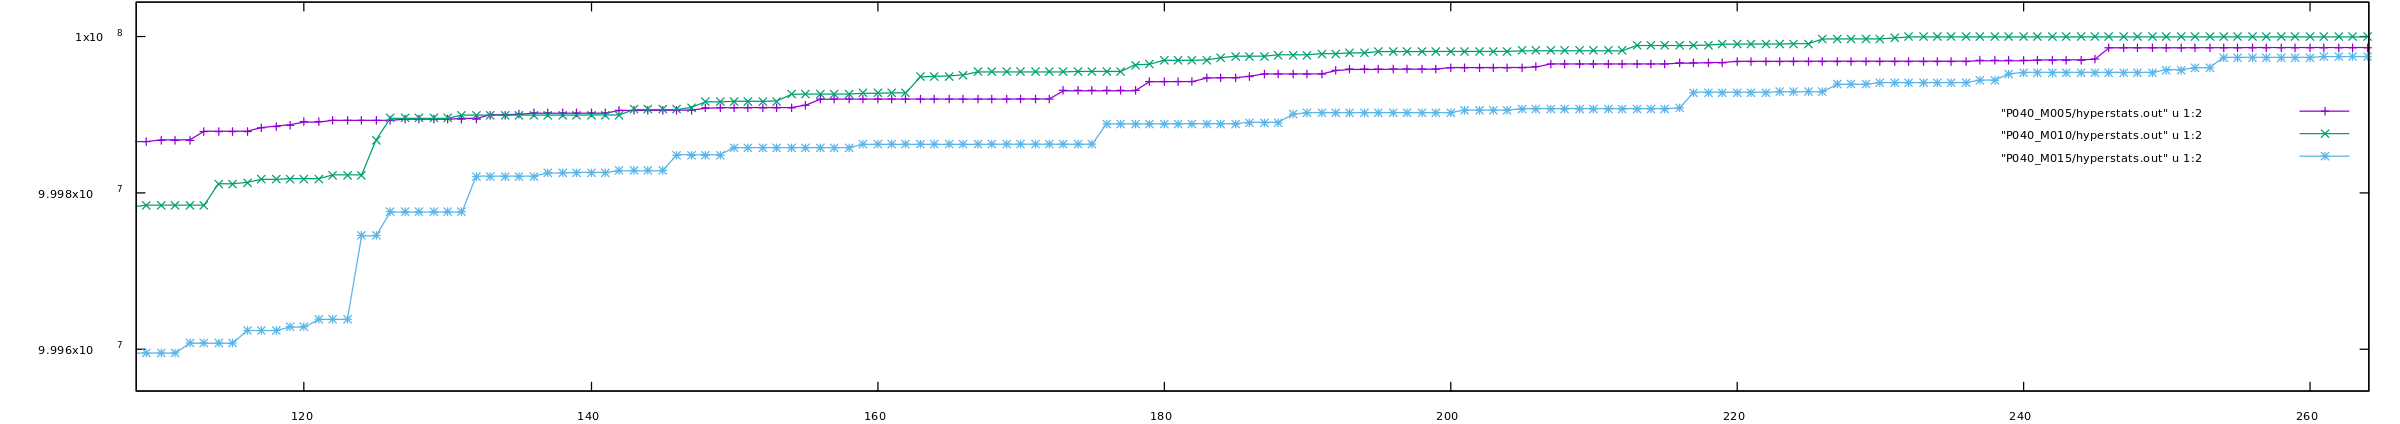
\includegraphics[width=\textwidth]{PopulationSize40.png}
  \caption{Population Size: 40}
  \label{fig:Population Size: 40 individuals}
\end{figure}
\begin{figure}[h]
  \centering
  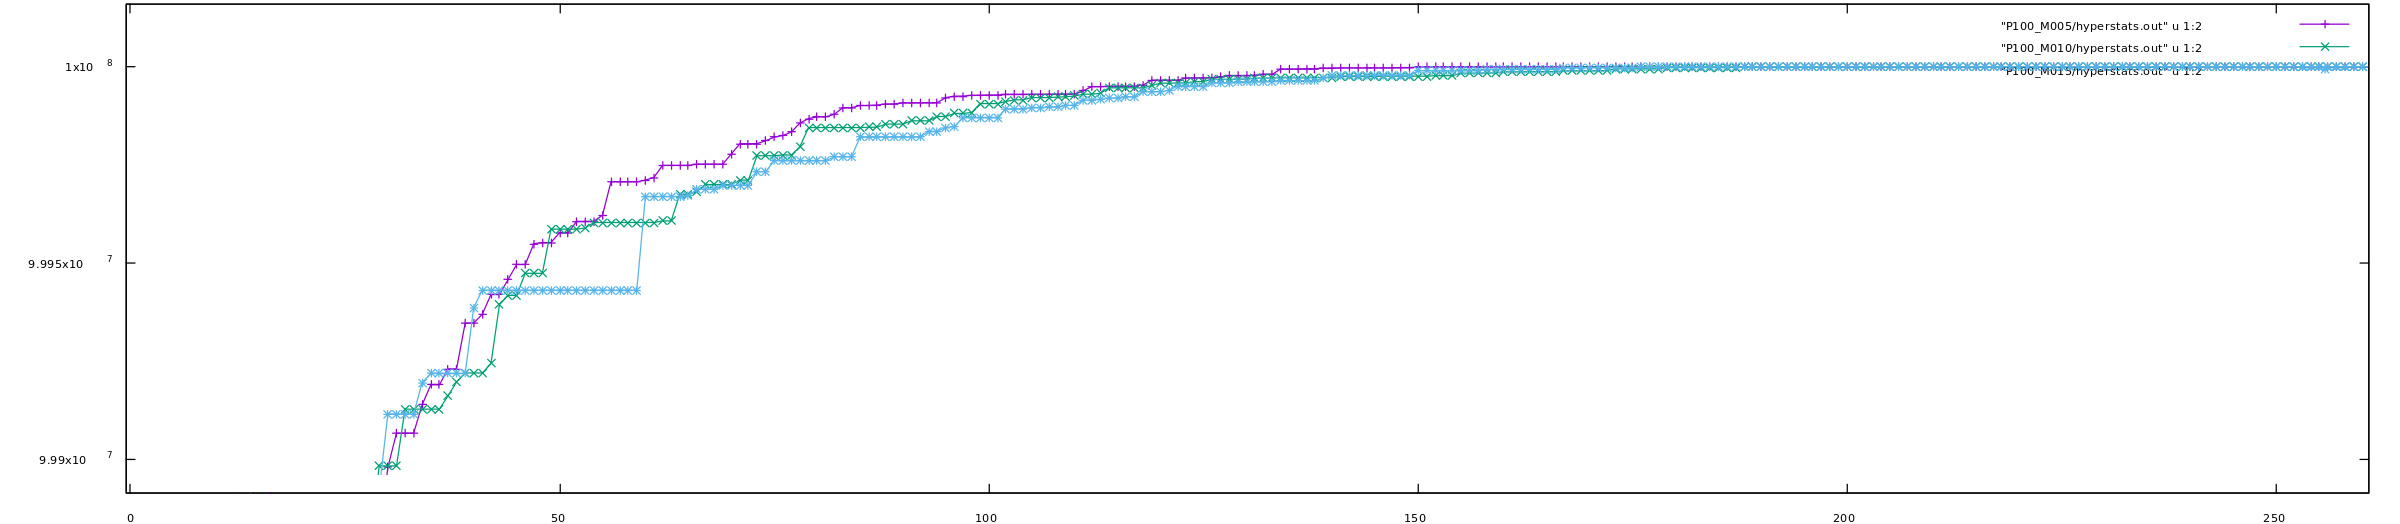
\includegraphics[width=\textwidth]{PopulationSize100.png}
  \caption{Population Size: 100}
  \label{fig:Population Size: 100 individuals}
  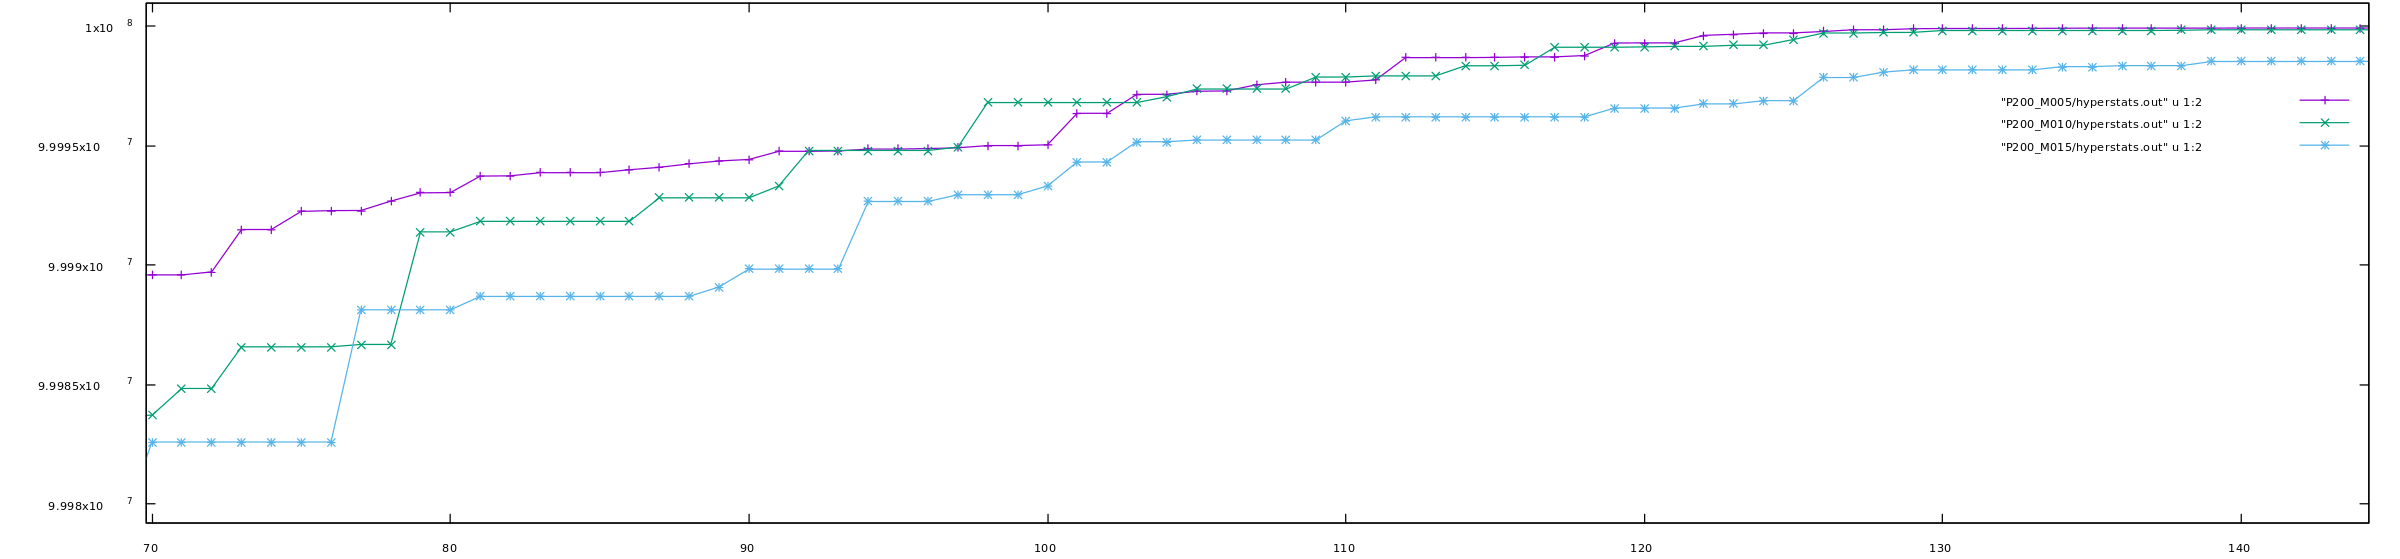
\includegraphics[width=\textwidth]{PopulationSize200.png}
  \caption{Population Size: 200}
  \label{fig:PopulationSize200}
\end{figure}
\begin{figure}[h]
  \centering
  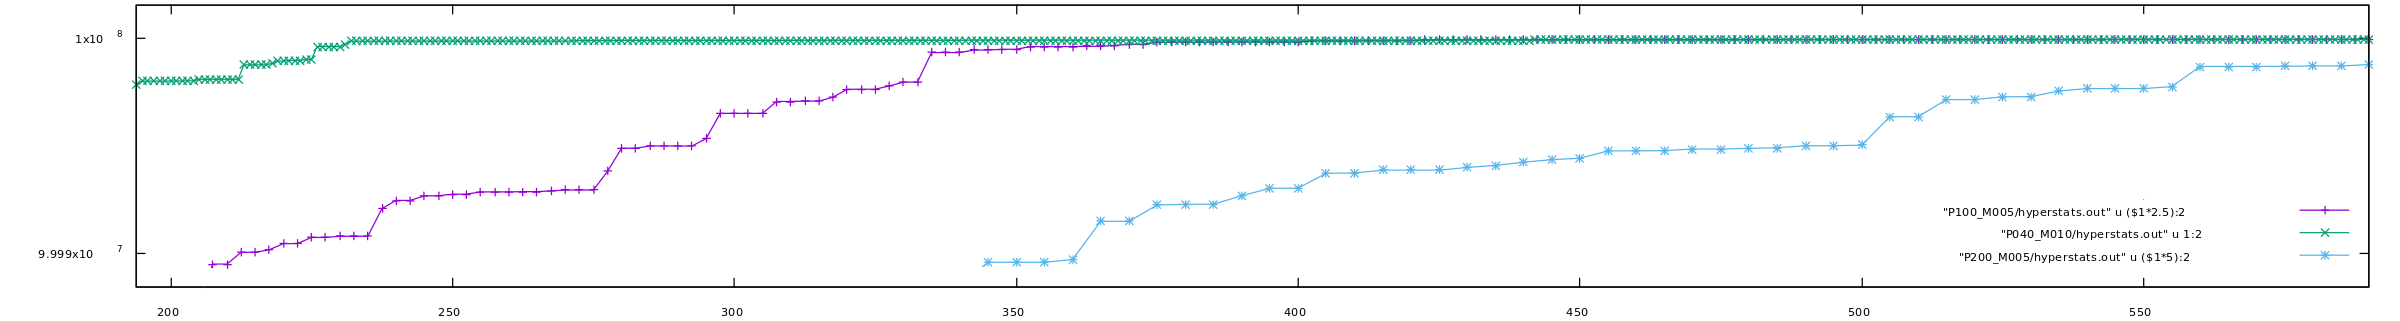
\includegraphics[width=\textwidth]{BestMutationRatePerPopulationSize.png}
  \caption{Best Mutation Rate per Population Size}
  \label{fig:BestMutationRateperPopulationSize}
\end{figure}
\newpage
\hbox{
In Figure \ref{fig:BestMutationRateperPopulationSize}, the comparison is shown for the best \textbf{Mutation Rate} for each \textbf{Population Size}.\\
}
\begin{itemize}
  \item PS: 40, MR: 0.10
  \item PS: 100, MR: 0.05
  \item PS: 200, MR: 0.05
\end{itemize}
The combination of a \textbf{Population Size} of 40 individuals and a \textbf{Mutation Rate} of 0.10 turns out to be the best.\\

\subsection{Final generation's non-dominated solution sets}
For each Population Size is possible to see 3 different Figure (for each Mutation Rate) of the final generation's non-dominated solution set. It's an approximate finite representation of the optimal solutions forming the Pareto frontier.\\
The quantity of points depicted is influenced by the population size, meaning that experiments with larger populations yield a denser and more continuous non-dominated frontier.\\

\textbf{Population Size of 40 individuals}
\begin{figure}[h]
    \centering
    \begin{minipage}{0.49\textwidth}
        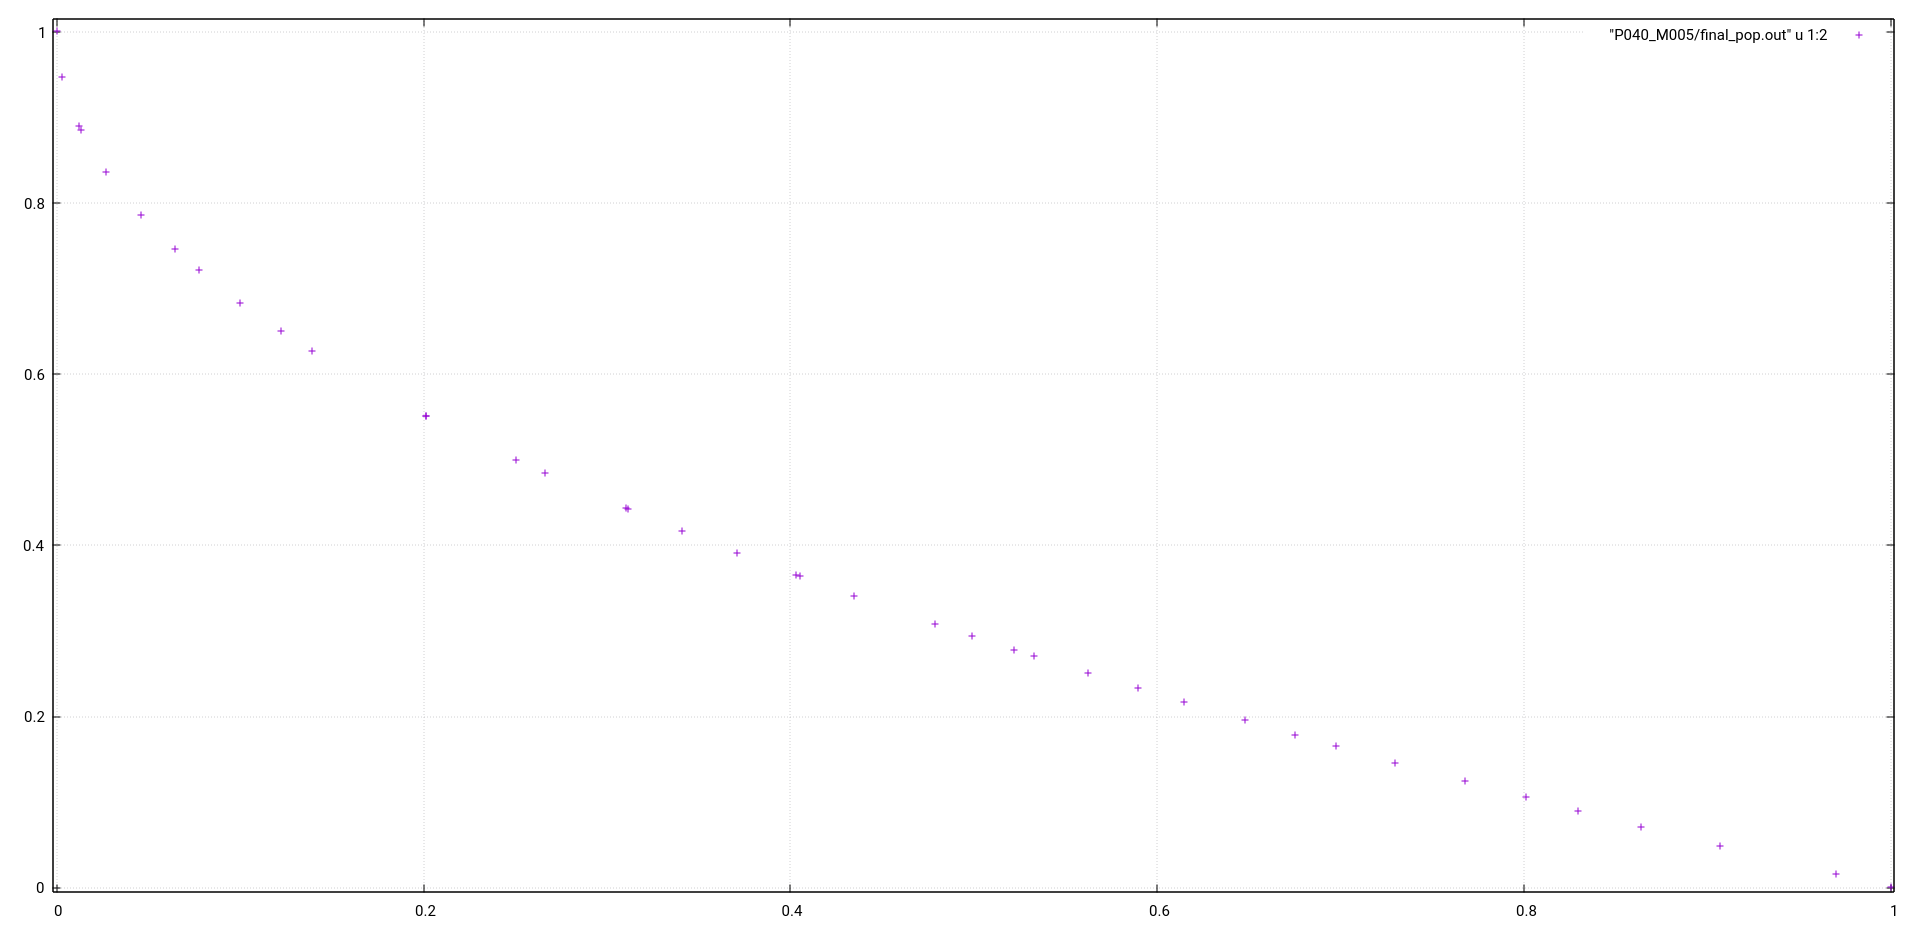
\includegraphics[width=\linewidth]{population_plot/P040_M005.png}
        \caption{Mutation Rate: 0.05}
        \label{fig:P040_M005}
    \end{minipage}
    \hfill
    \begin{minipage}{0.49\textwidth}
        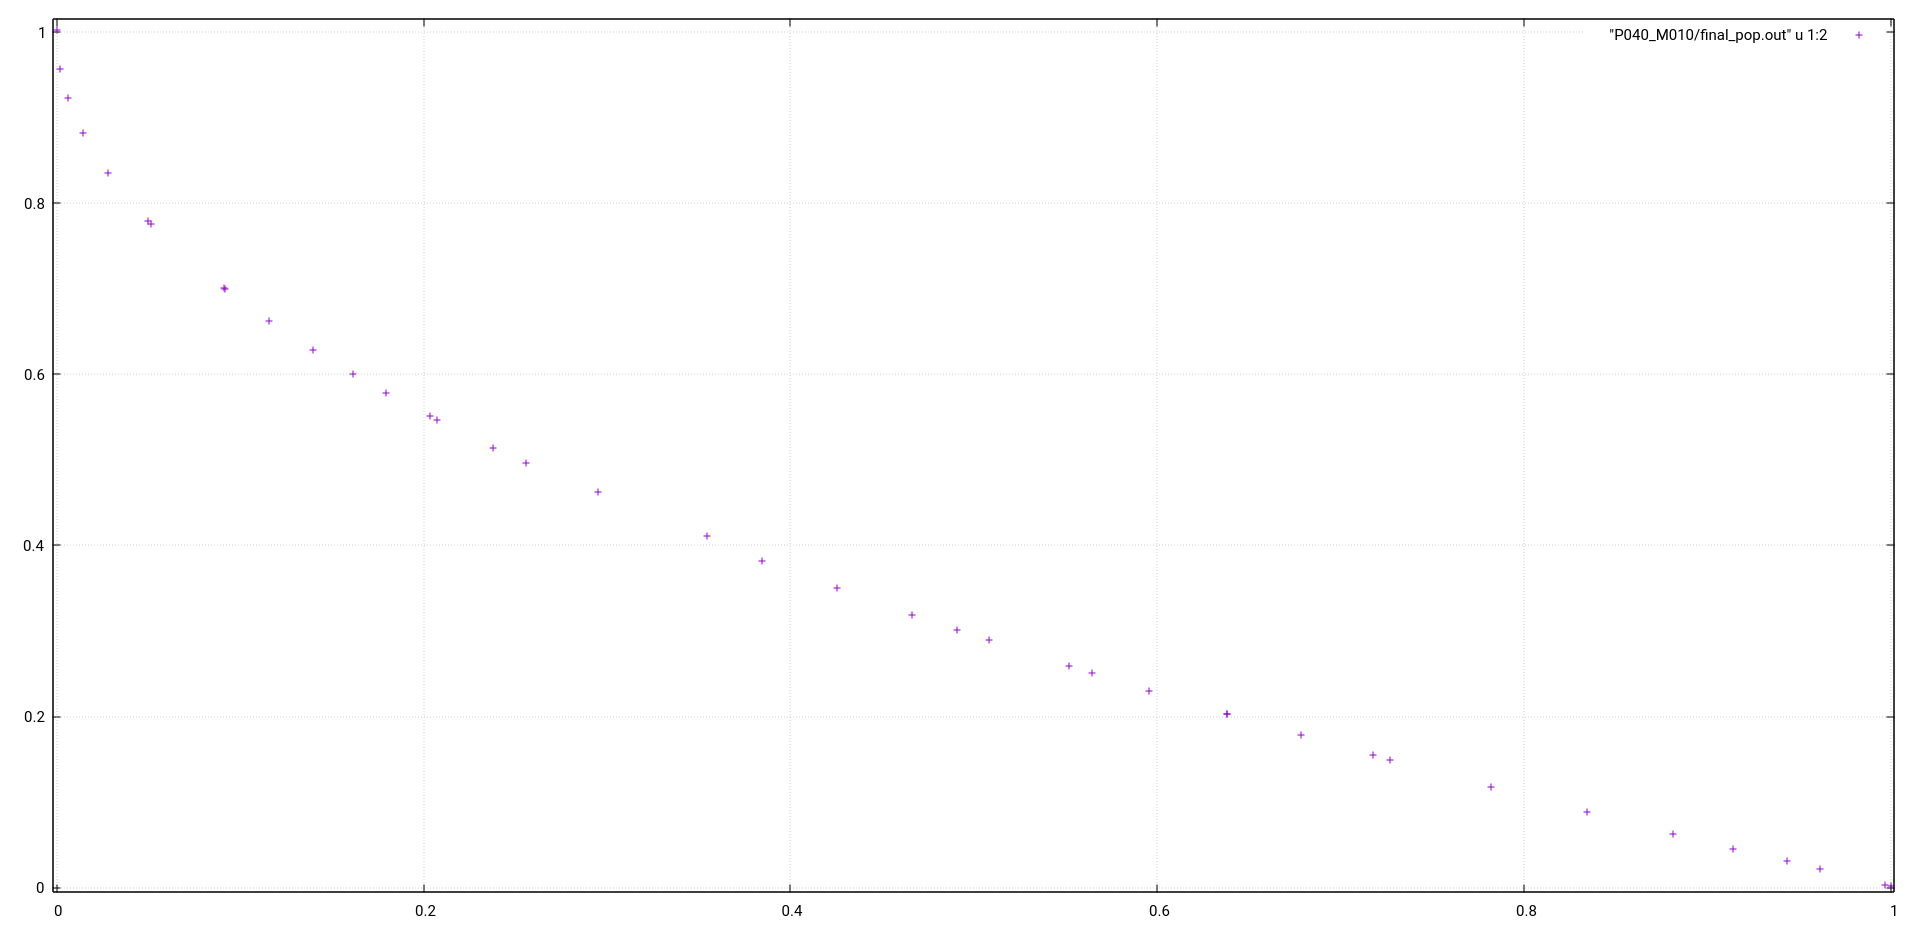
\includegraphics[width=\linewidth]{population_plot/P040_M010.png}
        \caption{Mutation Rate: 0.10}
        \label{fig:P040_M010}
    \end{minipage}
\end{figure}
\begin{figure}[h]
    \centering
    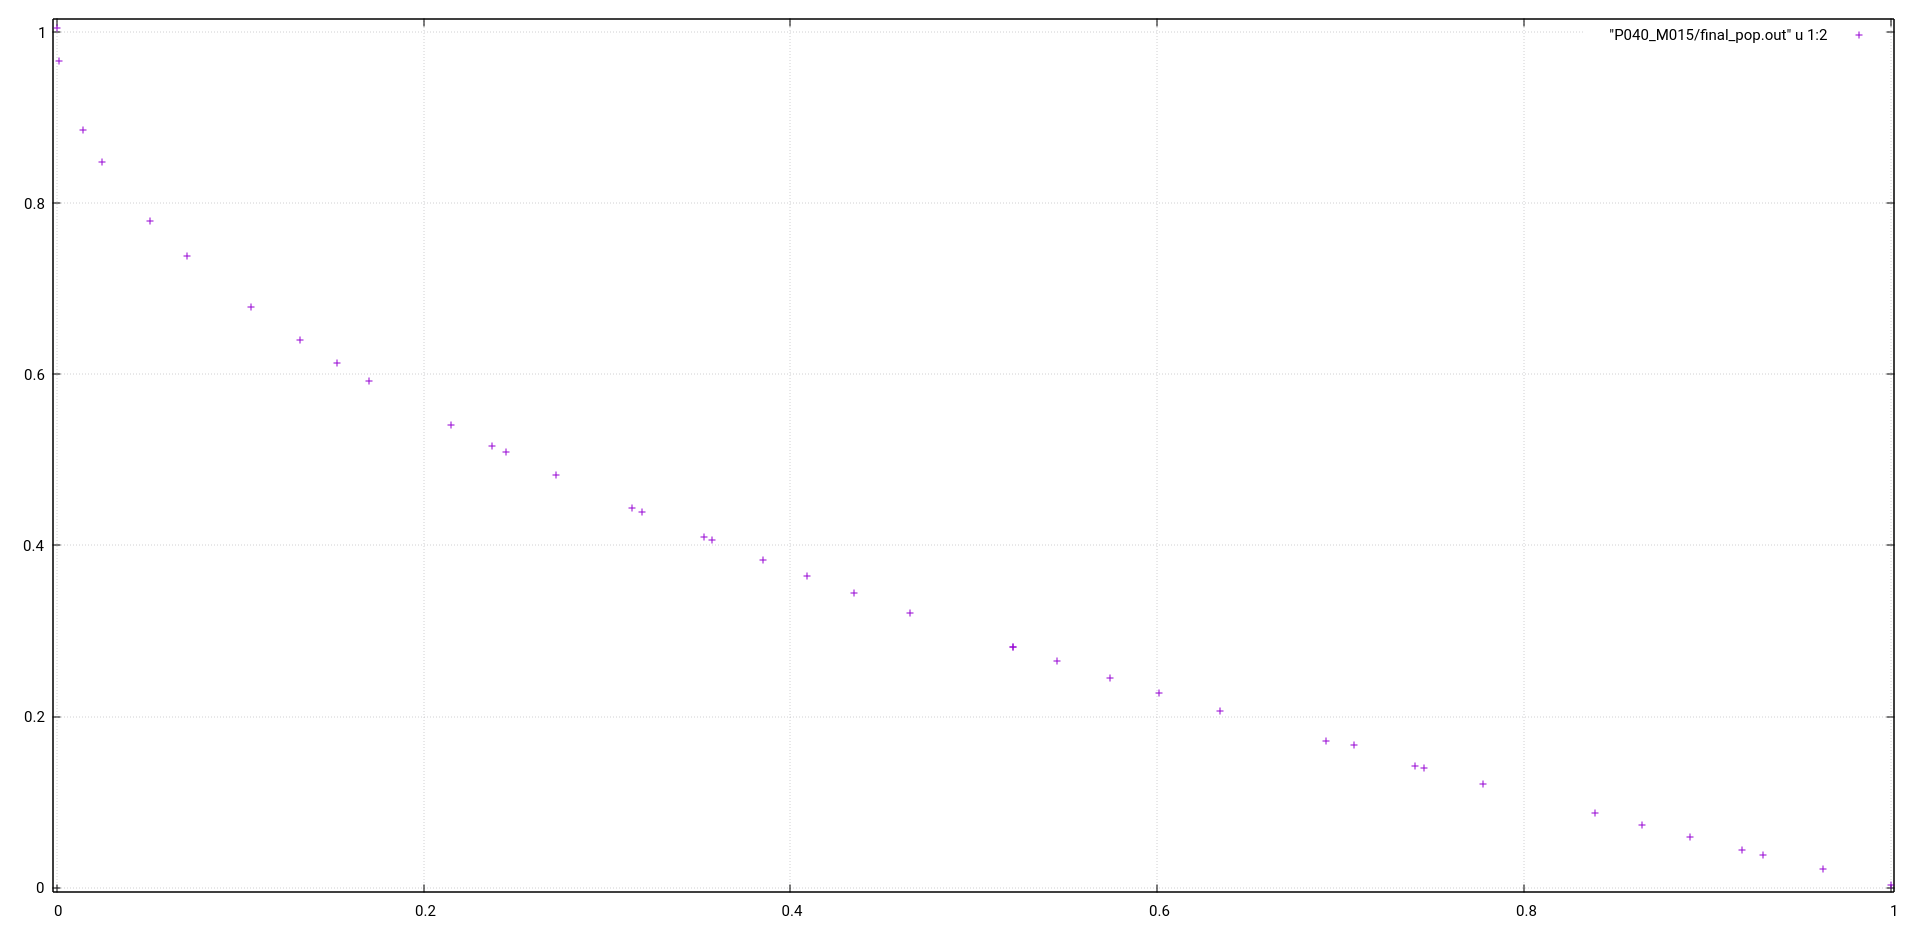
\includegraphics[width=0.49\linewidth]{population_plot/P040_M015.png}
    \caption{Mutation Rate: 0.15}
    \label{fig:P040_M015}
\end{figure}

\newpage

\textbf{Population Size of 100 individuals}
\begin{figure}[h]
    \centering
    \begin{minipage}{0.49\textwidth}
        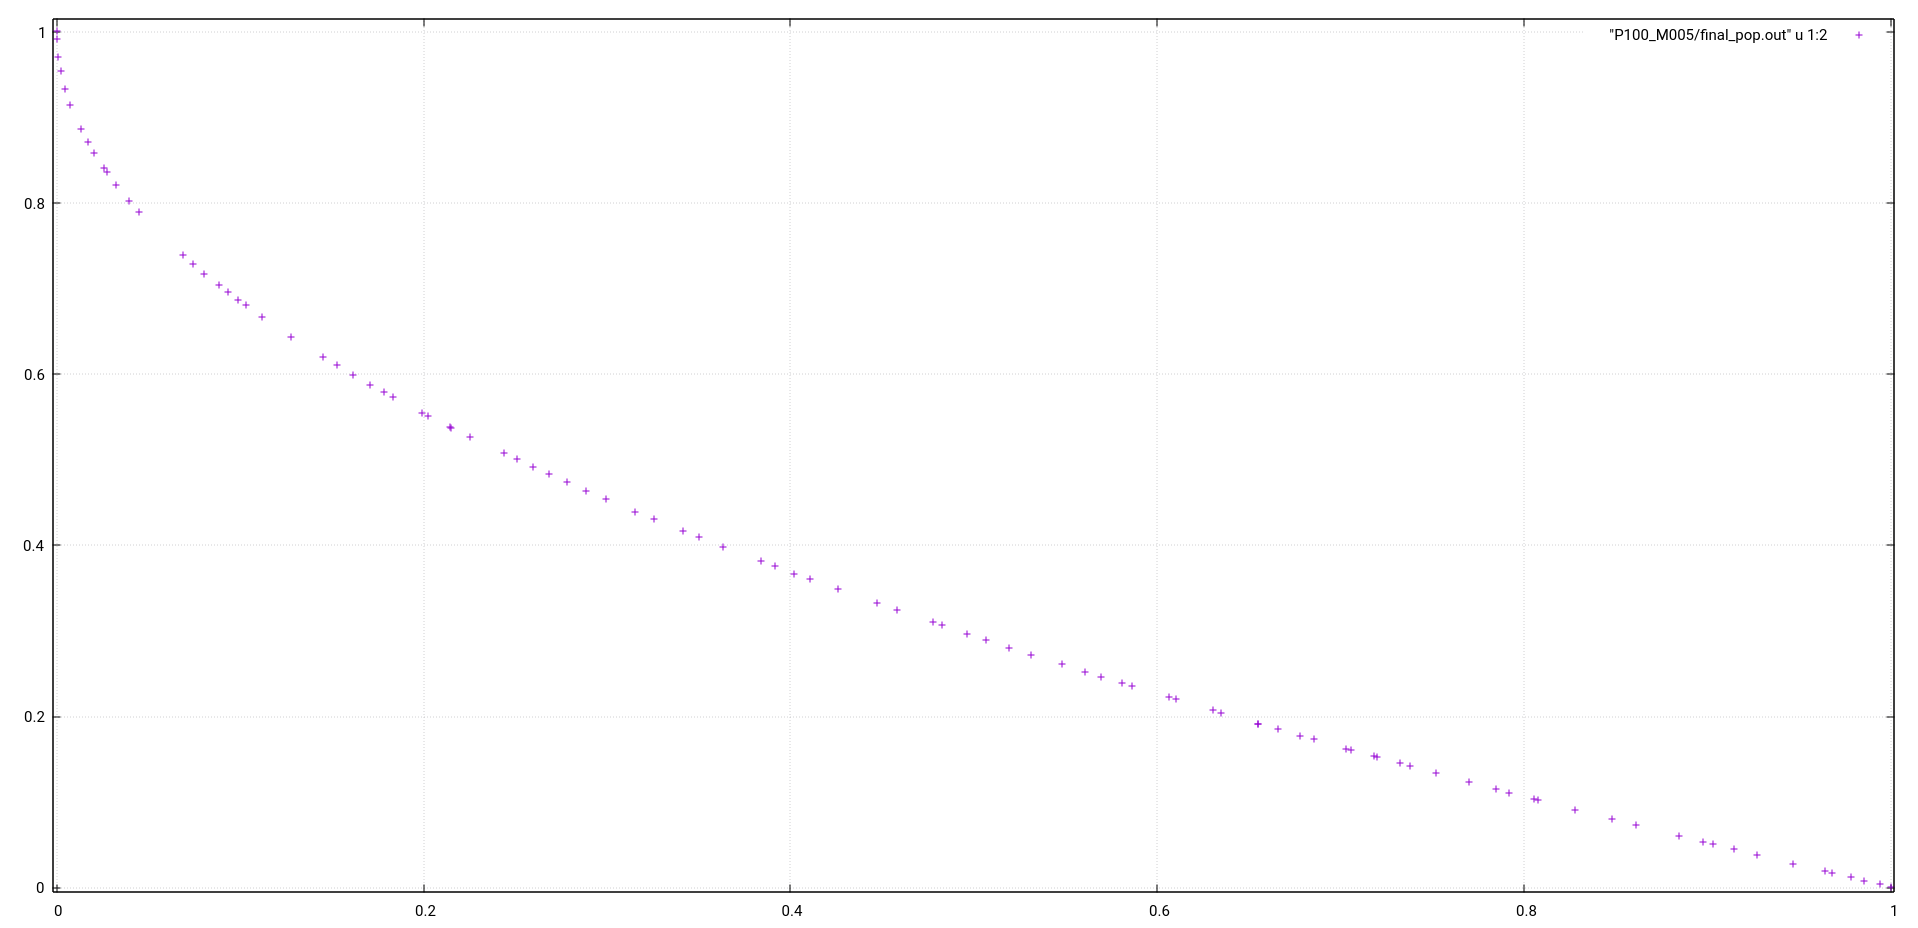
\includegraphics[width=\linewidth]{population_plot/P100_M005.png}
        \caption{Mutation Rate: 0.05}
        \label{fig:P100_M005}
    \end{minipage}
    \hfill
    \begin{minipage}{0.49\textwidth}
        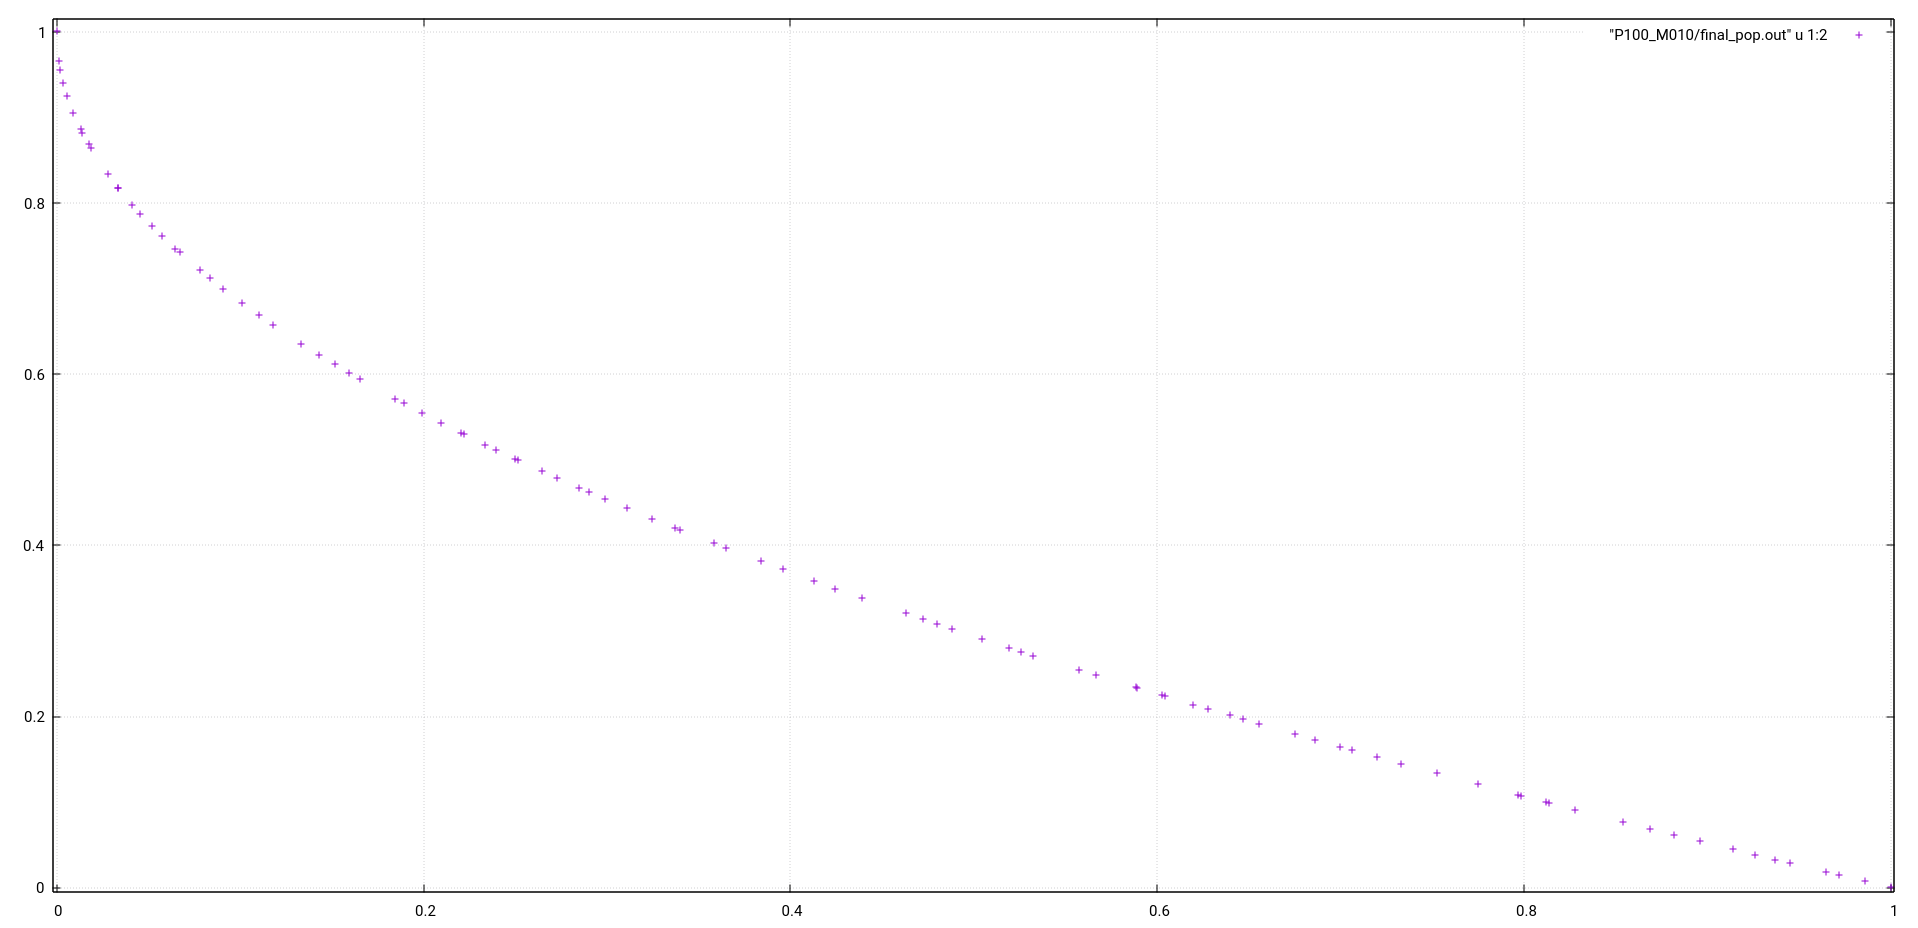
\includegraphics[width=\linewidth]{population_plot/P100_M010.png}
        \caption{Mutation Rate: 0.10}
        \label{fig:P100_M010}
    \end{minipage}
\end{figure}

\begin{figure}[h]
    \centering
    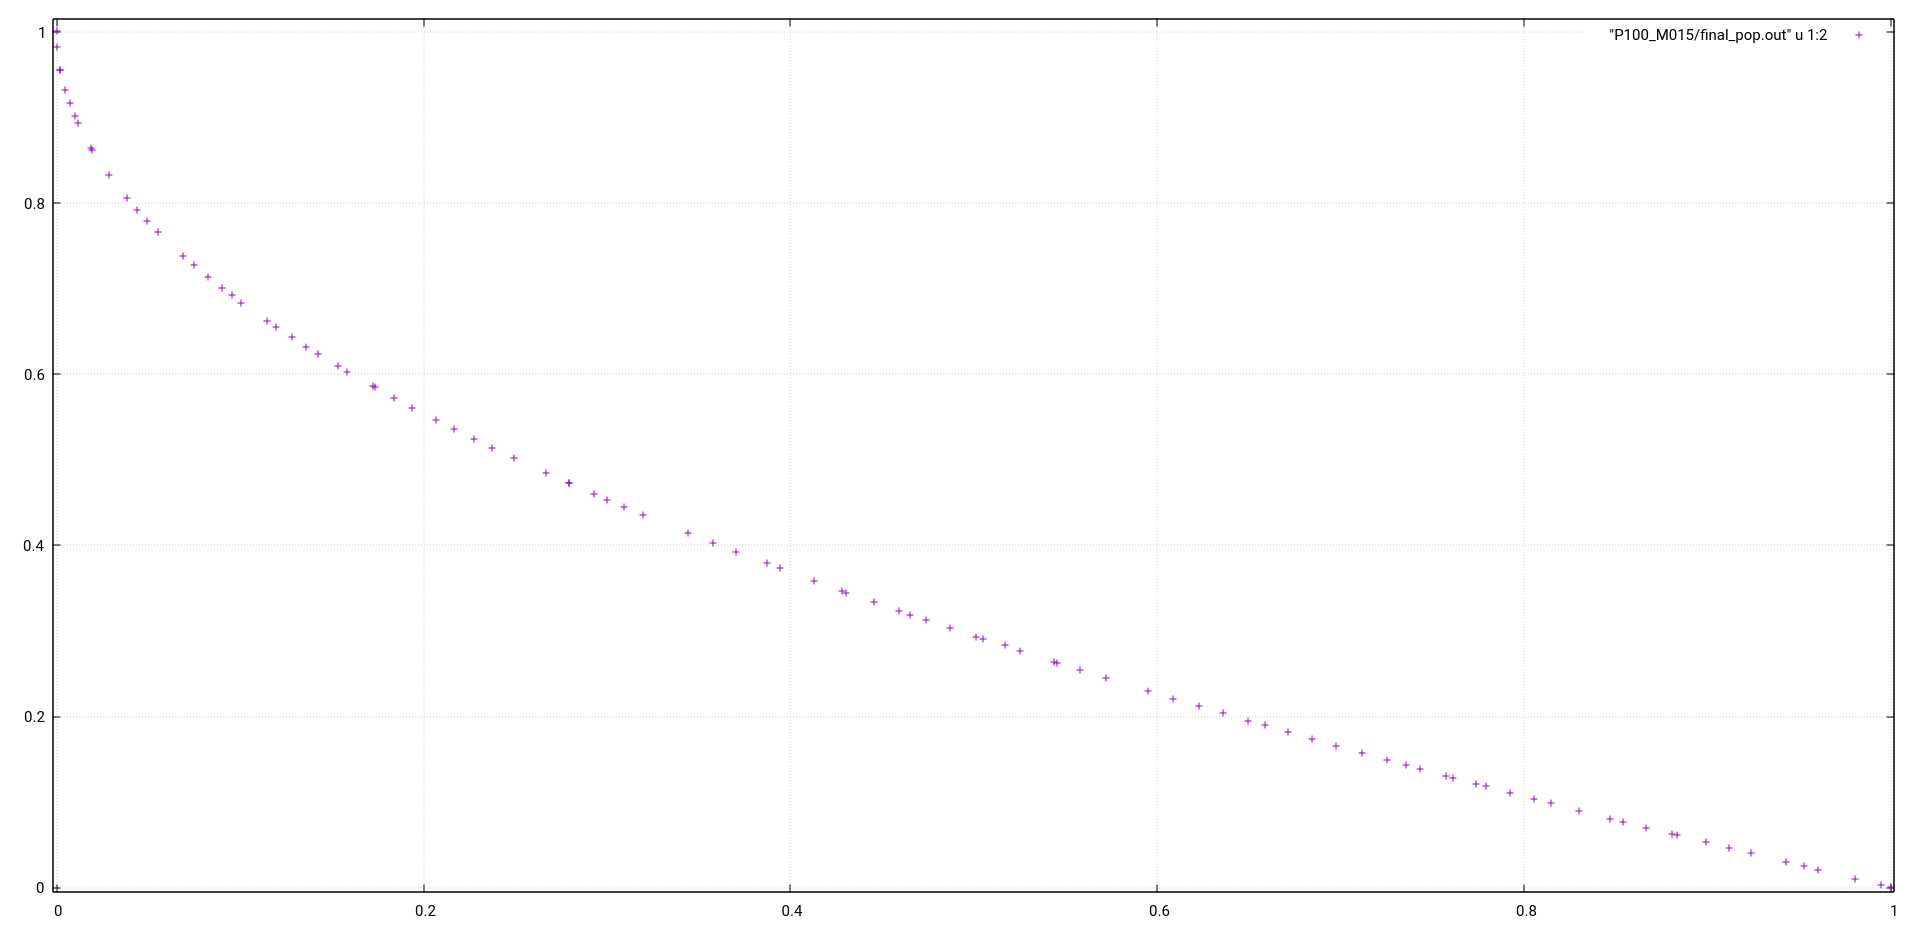
\includegraphics[width=0.49\linewidth]{population_plot/P100_M015.png}
    \caption{Mutation Rate: 0.15}
    \label{fig:P100_M015}
\end{figure}

\newpage

\textbf{Population Size of 200 individuals}
\begin{figure}[h]
    \centering
    \begin{minipage}{0.49\textwidth}
        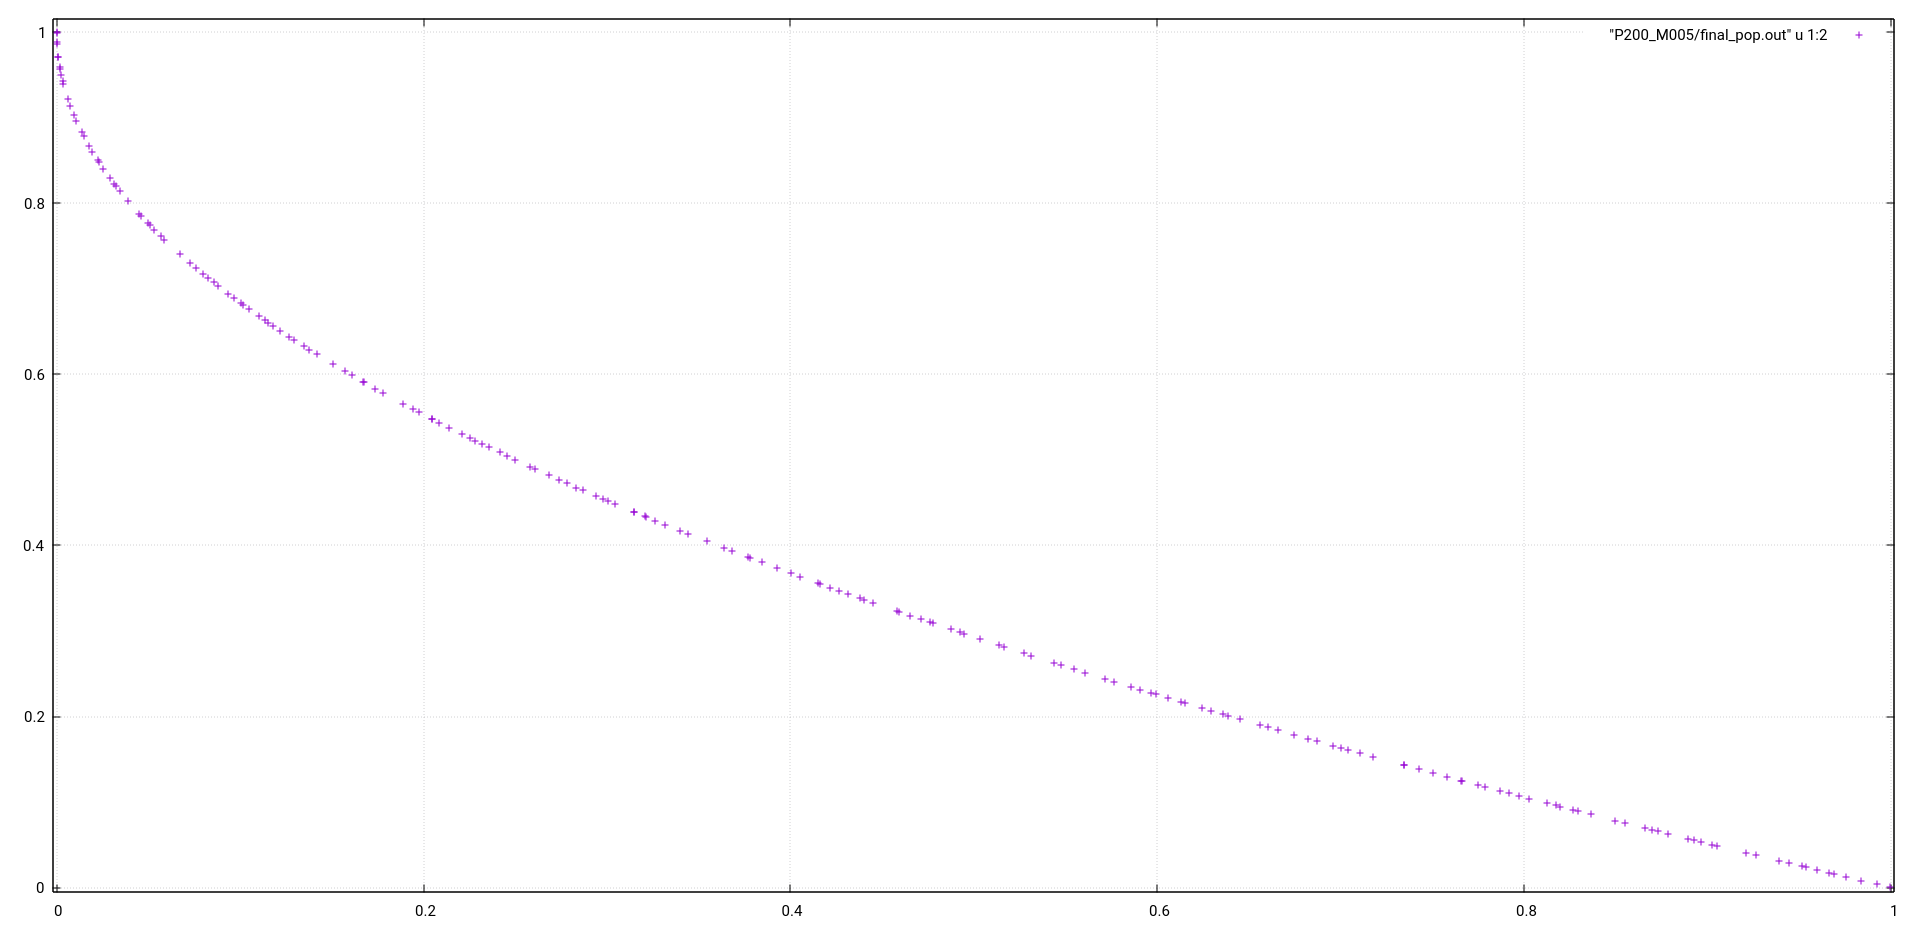
\includegraphics[width=\linewidth]{population_plot/P200_M005.png}
        \caption{Mutation Rate: 0.05}
        \label{fig:P200_M005}
    \end{minipage}
    \hfill
    \begin{minipage}{0.49\textwidth}
        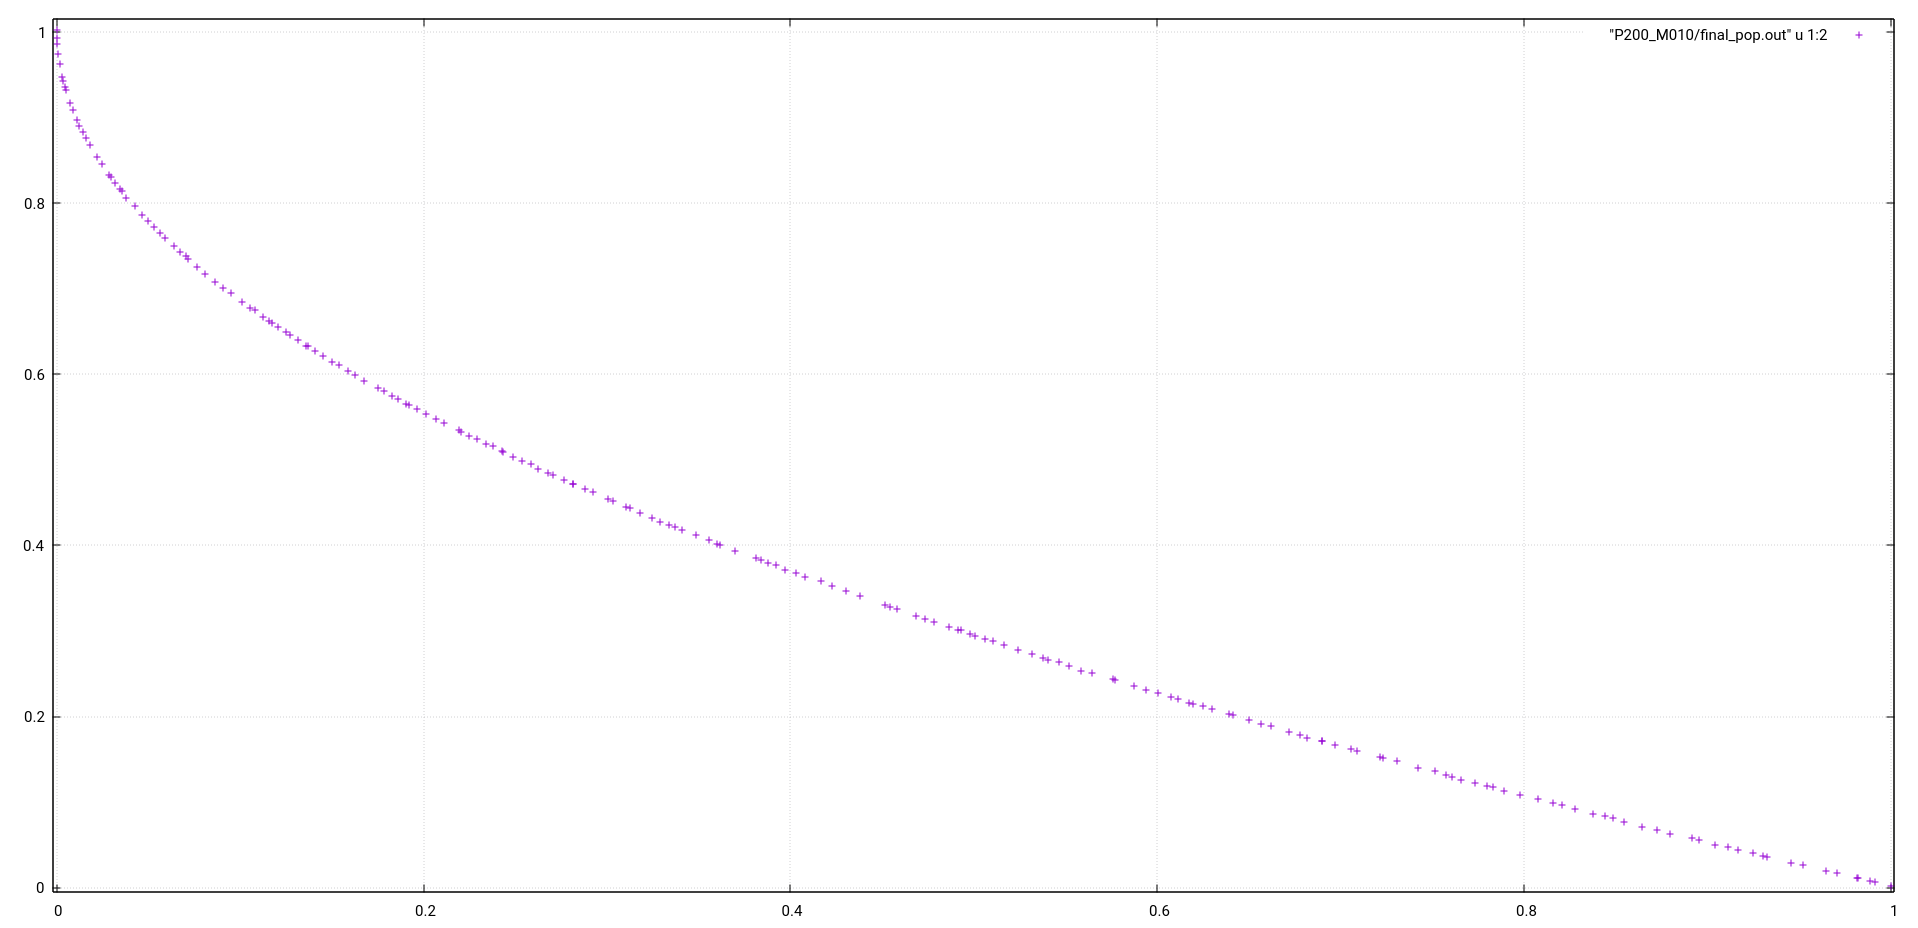
\includegraphics[width=\linewidth]{population_plot/P200_M010.png}
        \caption{Mutation Rate: 0.10}
        \label{fig:P200_M010}
    \end{minipage}
\end{figure}

\begin{figure}[h]
    \centering
    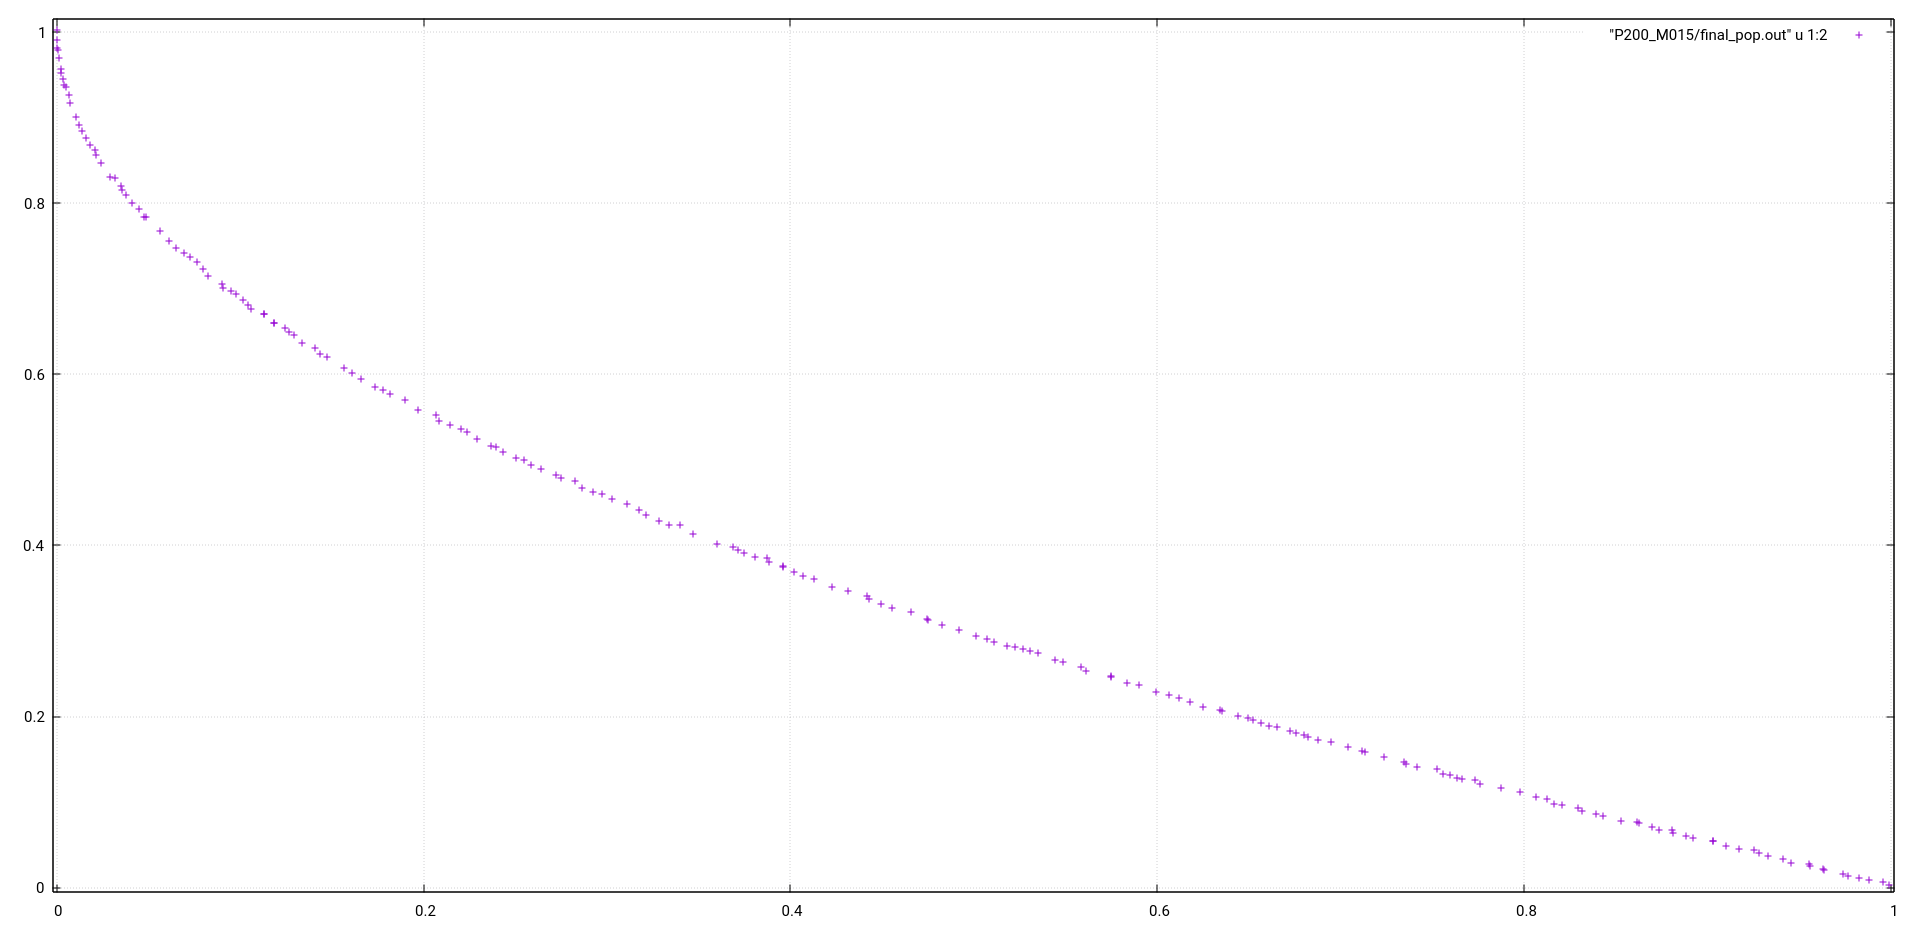
\includegraphics[width=0.49\linewidth]{population_plot/P200_M015.png}
    \caption{Mutation Rate: 0.15}
    \label{fig:P200_M015}
\end{figure}

\section*{Conclusion}
In this report, the application of the nondominated sorting genetic algorithm (NSGA-II) to solve the ZD4 problem through multiobjective evolutionary optimization was thoroughly explored. The impact of varying population sizes and mutation rates on the algorithm's convergence performance, with a specific focus on achieving a balance between exploration and exploitation, was examined.\\
A population size of 40 individuals coupled with a mutation rate of 0.10 yielded the most favorable results. These parameters resulted in a convergence pattern that effectively balanced exploring the solution space and exploiting promising regions.


\end{document}